% Лабораторная работа №1. Метод конечных разностей для ОДУ второго порядка.
\documentclass[12pt,a4paper]{article}

\usepackage[T2A]{fontenc}
\usepackage[utf8]{inputenc}
\usepackage[russian]{babel}

\usepackage{amsmath,amssymb}
\usepackage{graphicx}
\usepackage{booktabs}
\usepackage{array}
\usepackage[left=2.5cm,right=2cm,top=2.5cm,bottom=2.5cm]{geometry}
\usepackage{caption}
\usepackage{listings}
\usepackage{xcolor}
\usepackage[hidelinks]{hyperref}

\captionsetup[table]{position=top,justification=raggedleft,
                     singlelinecheck=false,labelsep=period}
\captionsetup[figure]{position=bottom,justification=centering,
                      singlelinecheck=false,labelsep=period}

\lstset{basicstyle=\ttfamily\footnotesize,
        keywordstyle=\color{black}\bfseries,
        columns=fullflexible,
        breaklines=true,
        frame=single,
        framerule=0.3pt,
        showstringspaces=false,
        language=Python}

\newcommand{\norm}[1]{\left\|#1\right\|}
\renewcommand{\arraystretch}{1.15}

\newcommand{\Discipline}{Конечно-разностные и сеточные методы}
\newcommand{\WorkKind}{ЛАБОРАТОРНАЯ РАБОТА №\,1}
\newcommand{\WorkTitleA}{Метод конечных разностей для обыкновенного}
\newcommand{\WorkTitleB}{дифференциального уравнения второго порядка}
\newcommand{\StudentGroup}{5030102/30101}
\newcommand{\StudentName}{Андреев Даниил}
\newcommand{\TeacherLabel}{Проверил:}
\newcommand{\TeacherName}{Елисеев А. А.}
\newcommand{\WorkYear}{2026}

\begin{document}

\begin{titlepage}
\color{titlecol}
\centering
\bfseries

\vspace*{18mm}

Министерство науки и высшего образования Российской Федерации\\[2mm]
{\large Санкт-Петербургский политехнический университет Петра Великого}\\[2mm]
Физико-Механический институт\\[2mm]

\vfill

{\Large \WorkKind}\\[3mm]
{\normalsize\mdseries по дисциплине «\Discipline»}\\[10mm]

{\large\mdseries \WorkTitleA\\[1.5mm] \WorkTitleB}

\vfill
\vfill

\hspace*{0.18\textwidth}%
\begin{minipage}{0.72\textwidth}
\mdseries
\begin{tabular}{@{}l@{\hspace{4mm}}l@{}}
Выполнил: & студент группы \StudentGroup\\
          & \StudentName\\[4mm]
\TeacherLabel & \TeacherName\\
\end{tabular}
\end{minipage}

\vfill

{\large Санкт-Петербург — \WorkYear}

\vspace*{10mm}
\end{titlepage}

\tableofcontents
\newpage

\section{Постановка задачи}

Рассматривается краевая задача третьего рода для линейного
обыкновенного дифференциального уравнения второго порядка:
\begin{equation}\label{eq:general}
\begin{aligned}
(Au)(x) &:= -\frac{d^2u}{dx^2} + p(x)\,\frac{du}{dx} + q(x)\,u = f(x),
   && x\in[a,b],\\[1mm]
(Au)(a) &:= -\alpha_a\,\frac{du}{dx}(a) + \beta_a\,u(a) = \gamma_a,
   && \beta_a\ge 0,\\[1mm]
(Au)(b) &:= \alpha_b\,\frac{du}{dx}(b) + \beta_b\,u(b) = \gamma_b,
   && \beta_b\ge 0,
\end{aligned}
\end{equation}
где
\begin{equation}\label{eq:cond}
q(x)\ge c>0,\qquad p(x),\,q(x)\neq \mathrm{const},\qquad
\alpha_a^2+\alpha_b^2\neq 0 .
\end{equation}
При этих условиях и $f\in C^2[a,b]$ задача имеет единственное решение
$u\in C^4[a,b]$.

Чтобы можно было измерять погрешность численного решения, задача
строится по известному ответу. Выбирается функция $u^*\in C^4[a,b]$ и
вычисляются согласованные с ней правые части
\begin{equation}\label{eq:manufactured}
f^*(x):=(Au^*)(x),\qquad
\gamma^*_a:=(Au^*)(a),\qquad
\gamma^*_b:=(Au^*)(b).
\end{equation}
Решается задача
\begin{equation}\label{eq:test}
\left\{
\begin{aligned}
(Au)(x) &= f^*(x),\\
(Au)(a) &= \gamma^*_a,\\
(Au)(b) &= \gamma^*_b,
\end{aligned}
\right.
\end{equation}
точное решение которой, очевидно, $u=u^*$.

\subsection{Выбранные данные}

В работе принято
\begin{equation}\label{eq:data}
[a,b]=[0,\,2],\qquad
p(x)=2+\cos\pi x,\qquad
q(x)=1+x^2,
\end{equation}
\begin{equation}\label{eq:bc}
\alpha_a=1,\quad \beta_a=1,\qquad
\alpha_b=1,\quad \beta_b=2 .
\end{equation}
Условия~\eqref{eq:cond} выполнены: $q(x)\ge 1>0$, функции $p$ и $q$ не
постоянны, $\beta_a,\beta_b\ge 0$ и $\alpha_a^2+\alpha_b^2=2\neq 0$.
Оба краевых условия --- третьего рода, поэтому способ их аппроксимации
влияет на порядок точности схемы.

В качестве точного решения взято
\begin{equation}\label{eq:ustar}
u^*(x)=x\sin 2\pi x + e^{-x}.
\end{equation}
На отрезке $[0,2]$ эта функция имеет четыре внутренних экстремума,
амплитуда колебаний растёт с $x$, а слагаемое $e^{-x}$ даёт участок
медленного изменения у левого конца (рис.~\ref{fig:exact}). Её
производные
\begin{align}
{u^*}'(x)  &= \sin 2\pi x + 2\pi x\cos 2\pi x - e^{-x},\\
{u^*}''(x) &= 4\pi\cos 2\pi x - 4\pi^2 x\sin 2\pi x + e^{-x},
\end{align}
откуда по формулам~\eqref{eq:manufactured}
\[
f^*(x)=-{u^*}''+p\,{u^*}'+q\,u^*,\qquad
\gamma^*_a=2,\qquad
\gamma^*_b=4\pi+e^{-2}\approx 12{,}70 .
\]

\begin{figure}[htbp]
\centering
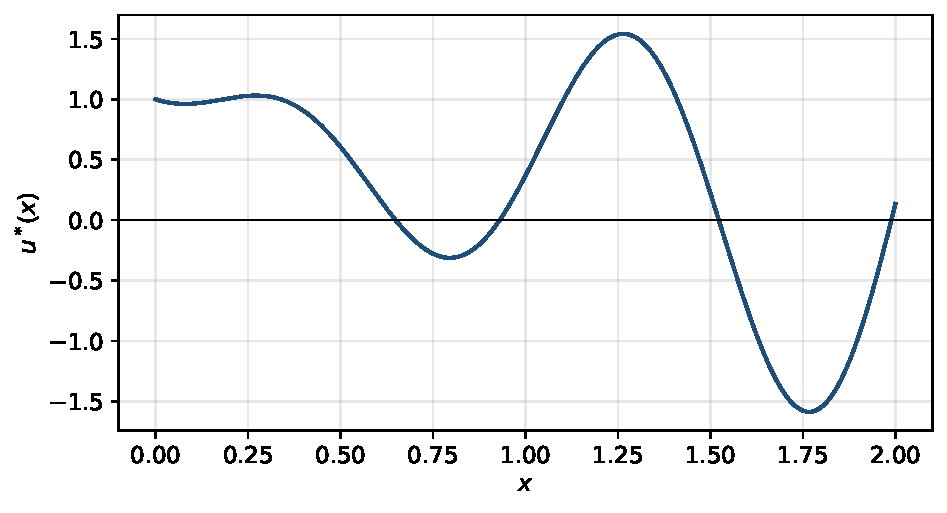
\includegraphics[width=0.85\textwidth]{figures/exact.pdf}
\caption{Точное решение $u^*(x)=x\sin 2\pi x+e^{-x}$}
\label{fig:exact}
\end{figure}

\section{Разностные схемы}

\subsection{Сетка}

Вводится равномерная сетка
\[
x_i=a+ih,\quad i=0,1,\dots,n,\qquad h=\frac{b-a}{n},
\]
обозначения: $p_i=p(x_i)$, $q_i=q(x_i)$, $f_i=f^*(x_i)$, $u_i=u^*(x_i)$.
Численное решение --- сеточная функция $v_h=(v_0,\dots,v_n)$.

\subsection{Внутренние узлы}

Во внутренних узлах $i=1,\dots,n-1$ обе схемы используют центральные
разности:
\begin{equation}\label{eq:inner}
-\frac{v_{i-1}-2v_i+v_{i+1}}{h^2}
+p_i\,\frac{v_{i+1}-v_{i-1}}{2h}
+q_i v_i = f_i .
\end{equation}
Оценим погрешность аппроксимации. Подставим в~\eqref{eq:inner} вместо
$v_i$ значения точного решения $u_i$ и разложим соседние узлы по формуле
Тейлора в точке $x_i$:
\begin{equation}\label{eq:taylor_inner}
u_{i\pm1}=u_i\pm h\,u'_i+\frac{h^2}{2}u''_i
          \pm\frac{h^3}{6}u'''_i+\frac{h^4}{24}u^{(4)}_i+O(h^5).
\end{equation}
Складывая и вычитая эти два разложения, получаем
\begin{equation}\label{eq:d2}
\frac{u_{i-1}-2u_i+u_{i+1}}{h^2}=u''_i+\frac{h^2}{12}u^{(4)}_i+O(h^4),
\end{equation}
\begin{equation}\label{eq:d1}
\frac{u_{i+1}-u_{i-1}}{2h}=u'_i+\frac{h^2}{6}u'''_i+O(h^4).
\end{equation}
Существенно, что в обеих формулах члены с нечётными степенями $h$
сократились: в~\eqref{eq:d2} --- нечётные производные (разложения
складываются), в~\eqref{eq:d1} --- чётные (разложения вычитаются). Это
свойство симметрии центральных разностей, поэтому в остатке стоят только
чётные степени $h$.

Подставляя~\eqref{eq:d2} и~\eqref{eq:d1} в левую часть~\eqref{eq:inner} и
вычитая $f_i$, получаем невязку
\[
\psi_i=-u''_i-\frac{h^2}{12}u^{(4)}_i
       +p_iu'_i+p_i\frac{h^2}{6}u'''_i+q_iu_i-f_i .
\]
Слагаемые без $h$ дают $-u''_i+p_iu'_i+q_iu_i-f_i=0$, так как точное
решение удовлетворяет уравнению. Остаётся
\begin{equation}\label{eq:psi}
\psi_i = -\frac{h^2}{12}\,u^{(4)}(x_i)+p_i\,\frac{h^2}{6}\,u'''(x_i)+O(h^4)
       = O(h^2).
\end{equation}

Уравнения~\eqref{eq:inner} дают трёхдиагональную матрицу с элементами
\[
A_i=-\frac1{h^2}-\frac{p_i}{2h},\qquad
C_i=\frac2{h^2}+q_i,\qquad
B_i=-\frac1{h^2}+\frac{p_i}{2h}.
\]
Диагональное преобладание $|C_i|>|A_i|+|B_i|$ выполняется при
\begin{equation}\label{eq:dd}
h<\frac{2}{\max|p(x)|}=\frac{2}{3},
\end{equation}
что для всех использованных сеток верно ($h\le 0{,}1$). Это вместе с
$q_i>0$ обеспечивает устойчивость метода прогонки.

\subsection{Схема A: краевые условия первого порядка}
\label{sec:scheme1}

Производные в краевых условиях заменяются односторонними разностями:
\[
\frac{du}{dx}(a)\approx\frac{v_1-v_0}{h},\qquad
\frac{du}{dx}(b)\approx\frac{v_n-v_{n-1}}{h}.
\]
Их погрешность видна из разложения Тейлора. В левом конце
\[
u_1=u_0+h\,u'_0+\frac{h^2}{2}u''_0+O(h^3)
\quad\Longrightarrow\quad
\frac{u_1-u_0}{h}=u'_0+\frac{h}{2}u''_0+O(h^2),
\]
то есть
\begin{equation}\label{eq:onesided}
u'_0-\frac{u_1-u_0}{h}=-\frac{h}{2}\,u''_0+O(h^2)=O(h).
\end{equation}
Аналогично в правом конце $u_{n-1}=u_n-h\,u'_n+\tfrac{h^2}{2}u''_n+O(h^3)$,
откуда
\[
u'_n-\frac{u_n-u_{n-1}}{h}=+\frac{h}{2}\,u''_n+O(h^2)=O(h).
\]
Здесь, в отличие от~\eqref{eq:d1}, вычитается только одно разложение,
и член с $u''$ не сокращается --- отсюда первый порядок. Граничные
уравнения:
\begin{equation}\label{eq:bc1}
\begin{aligned}
\Bigl(\frac{\alpha_a}{h}+\beta_a\Bigr)v_0-\frac{\alpha_a}{h}\,v_1
   &= \gamma^*_a,\\
-\frac{\alpha_b}{h}\,v_{n-1}+\Bigl(\frac{\alpha_b}{h}+\beta_b\Bigr)v_n
   &= \gamma^*_b .
\end{aligned}
\end{equation}
Внутри области схема имеет второй порядок, но на границе --- первый,
поэтому вся схема сходится с первым порядком, $k=1$.

\subsection{Схема B: краевые условия второго порядка}
\label{sec:scheme2}

Чтобы повысить порядок на границе и сохранить трёхдиагональность,
используется разложение Тейлора с подстановкой самого уравнения. В левом
конце
\[
u_1=u_0+h\,u'_0+\frac{h^2}{2}u''_0+O(h^3)
\;\Longrightarrow\;
u'_0=\frac{u_1-u_0}{h}-\frac{h}{2}\,u''_0+O(h^2),
\]
а вторая производная берётся из уравнения в узле $x_0$:
$u''_0=p_0u'_0+q_0u_0-f_0$. Отсюда
\begin{equation}\label{eq:du_a}
u'_0=\frac{\dfrac{u_1-u_0}{h}-\dfrac{h}{2}\bigl(q_0u_0-f_0\bigr)}
          {1+\dfrac{h\,p_0}{2}}+O(h^2).
\end{equation}
Подставляя~\eqref{eq:du_a} в условие $-\alpha_a u'(a)+\beta_a u(a)=\gamma_a$
и умножая на $D_a=1+\tfrac{h p_0}{2}$, получаем
\begin{equation}\label{eq:bc2a}
\Bigl(\frac{\alpha_a}{h}+\frac{\alpha_a h q_0}{2}+\beta_a D_a\Bigr)v_0
-\frac{\alpha_a}{h}\,v_1
=\gamma^*_a D_a+\frac{\alpha_a h f_0}{2}.
\end{equation}
Аналогично в правом конце с $D_b=1-\tfrac{h p_n}{2}$:
\begin{equation}\label{eq:bc2b}
-\frac{\alpha_b}{h}\,v_{n-1}
+\Bigl(\frac{\alpha_b}{h}+\frac{\alpha_b h q_n}{2}+\beta_b D_b\Bigr)v_n
=\gamma^*_b D_b+\frac{\alpha_b h f_n}{2}.
\end{equation}
Теперь краевые условия аппроксимированы с точностью $O(h^2)$, как и
внутренние узлы, и схема сходится со вторым порядком, $k=2$.

\subsection{Решение системы и проверка программы}

Обе схемы дают систему с трёхдиагональной матрицей порядка $n+1$, которая
решается методом прогонки за $O(n)$ действий.

Программа проверялась на простом решении $u^*=x^2$. Схема B воспроизводит
его точно (отбрасываемые члены содержат $u'''$ и выше): получено
$\norm{z_h}\approx 3{,}6\cdot10^{-15}$ при $n=20$ и
$1{,}8\cdot10^{-15}$ при $n=40$. Схема A на том же решении даёт
$7{,}0\cdot10^{-2}$ и $3{,}5\cdot10^{-2}$, то есть ровно вдвое меньше при
удвоении $n$, что соответствует первому порядку.

\section{Измерение погрешности}

Погрешность численного решения --- сеточная функция
\begin{equation}
z_h:=u_h-v_h,\qquad
\norm{z_h}=\max_{0\le i\le n}|u_i-v_i|.
\end{equation}
Для сходящейся схемы порядка $k$ имеем $\norm{z_h}=O(h^k)$, а при малых
$h$
\begin{equation}\label{eq:asympt}
\norm{z_h}\approx C h^k .
\end{equation}
Логарифмируя~\eqref{eq:asympt}, получаем
\begin{equation}\label{eq:log}
-\lg\norm{z_h}\approx -\lg C + k\,(-\lg h),
\end{equation}
то есть при $h\to 0$ зависимость $-\lg\norm{z_h}$ от $-\lg h$ выходит на
прямую с угловым коэффициентом $k$. Взяты минус логарифмы, так как сами
аргументы --- малые числа.

Кроме графика считается эмпирический порядок точности по двум соседним
сеткам. Пусть $h_j=h_{j-1}/2$. Тогда из~\eqref{eq:asympt}
\[
\frac{\norm{z_{h_{j-1}}}}{\norm{z_{h_j}}}
\approx\frac{C h_{j-1}^{\,k}}{C h_j^{\,k}}
=\Bigl(\frac{h_{j-1}}{h_j}\Bigr)^{\!k}=2^k,
\]
--- неизвестная константа $C$ сокращается. Логарифмируя по основанию 2,
получаем
\begin{equation}\label{eq:order}
k_j=\log_2\frac{\norm{z_{h_{j-1}}}}{\norm{z_{h_j}}},
\qquad h_j=h_{j-1}/2 .
\end{equation}
Величина $k_j$ --- это и есть наблюдаемый порядок точности; если схема
работает так, как задумано, $k_j$ выходит на постоянное значение $k$.
Расчёты велись на сетках $n=20\cdot 2^{\,j}$, $j=0,\dots,13$, то есть от
$n=20$ до $n=163\,840$; шаг последовательно уменьшался в 2 раза.

\section{Результаты}

\subsection{Сходимость схем}

На рис.~\ref{fig:compare} показаны решения при $n=40$. Схема B уже
практически совпадает с точным решением, а схема A заметно смещена,
сильнее всего у левого конца отрезка.

\begin{figure}[htbp]
\centering
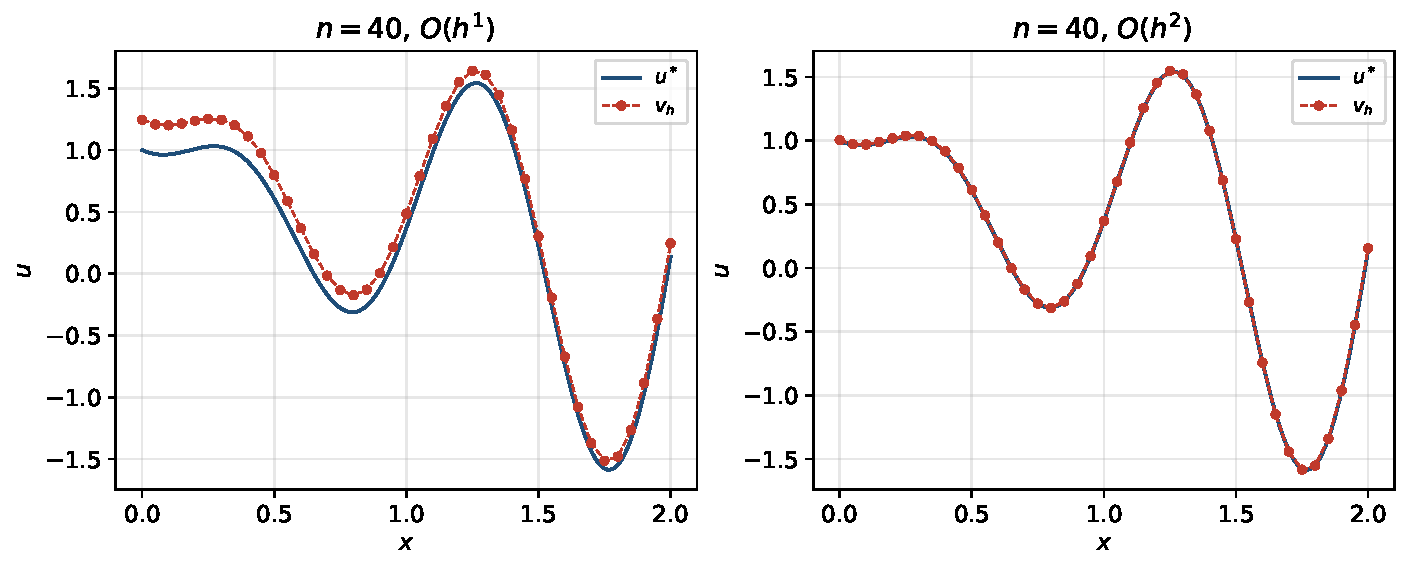
\includegraphics[width=\textwidth]{figures/compare.pdf}
\caption{Численное $v_h$ и точное $u^*$ решения при $n=40$:
слева схема $O(h)$, справа схема $O(h^2)$}
\label{fig:compare}
\end{figure}

Погрешности и эмпирические порядки приведены в табл.~\ref{tab:conv},
графики~\eqref{eq:log} --- на рис.~\ref{fig:conv}. Обе зависимости
ложатся на прямые, параллельные эталонным прямым с наклонами $k=1$ и
$k=2$. Эмпирический порядок равен $1{,}00$ для схемы A и $2{,}00$ для
схемы B; исключение --- последняя строка таблицы, о ней в
п.~\ref{sec:round}.

\begin{table}[htbp]
\caption{Погрешность $\norm{z_h}$ и эмпирический порядок точности $k$
(двойная точность)}
\label{tab:conv}
\centering
\begin{tabular}{r c c c c c}
\toprule
& & \multicolumn{2}{c}{схема A, $O(h)$} & \multicolumn{2}{c}{схема B, $O(h^2)$}\\
\cmidrule(lr){3-4}\cmidrule(lr){5-6}
$n$ & $h$ & $\norm{z_h}$ & $k$ & $\norm{z_h}$ & $k$\\
\midrule
20 & $1.00\cdot10^{-1}$ & $4.98\cdot10^{-1}$ & --- & $7.60\cdot10^{-2}$ & --- \\
40 & $5.00\cdot10^{-2}$ & $2.45\cdot10^{-1}$ & 1.02 & $1.89\cdot10^{-2}$ & 2.01 \\
80 & $2.50\cdot10^{-2}$ & $1.21\cdot10^{-1}$ & 1.01 & $4.73\cdot10^{-3}$ & 2.00 \\
160 & $1.25\cdot10^{-2}$ & $6.05\cdot10^{-2}$ & 1.01 & $1.18\cdot10^{-3}$ & 2.00 \\
320 & $6.25\cdot10^{-3}$ & $3.02\cdot10^{-2}$ & 1.00 & $2.95\cdot10^{-4}$ & 2.00 \\
640 & $3.13\cdot10^{-3}$ & $1.51\cdot10^{-2}$ & 1.00 & $7.38\cdot10^{-5}$ & 2.00 \\
1280 & $1.56\cdot10^{-3}$ & $7.53\cdot10^{-3}$ & 1.00 & $1.85\cdot10^{-5}$ & 2.00 \\
2560 & $7.81\cdot10^{-4}$ & $3.77\cdot10^{-3}$ & 1.00 & $4.61\cdot10^{-6}$ & 2.00 \\
5120 & $3.91\cdot10^{-4}$ & $1.88\cdot10^{-3}$ & 1.00 & $1.15\cdot10^{-6}$ & 2.00 \\
10240 & $1.95\cdot10^{-4}$ & $9.41\cdot10^{-4}$ & 1.00 & $2.88\cdot10^{-7}$ & 2.00 \\
20480 & $9.77\cdot10^{-5}$ & $4.71\cdot10^{-4}$ & 1.00 & $7.21\cdot10^{-8}$ & 2.00 \\
40960 & $4.88\cdot10^{-5}$ & $2.35\cdot10^{-4}$ & 1.00 & $1.79\cdot10^{-8}$ & 2.01 \\
81920 & $2.44\cdot10^{-5}$ & $1.18\cdot10^{-4}$ & 1.00 & $4.38\cdot10^{-9}$ & 2.03 \\
163840 & $1.22\cdot10^{-5}$ & $5.88\cdot10^{-5}$ & 1.00 & $3.54\cdot10^{-9}$ & 0.31 \\
\bottomrule
\end{tabular}
\end{table}

\begin{figure}[htbp]
\centering
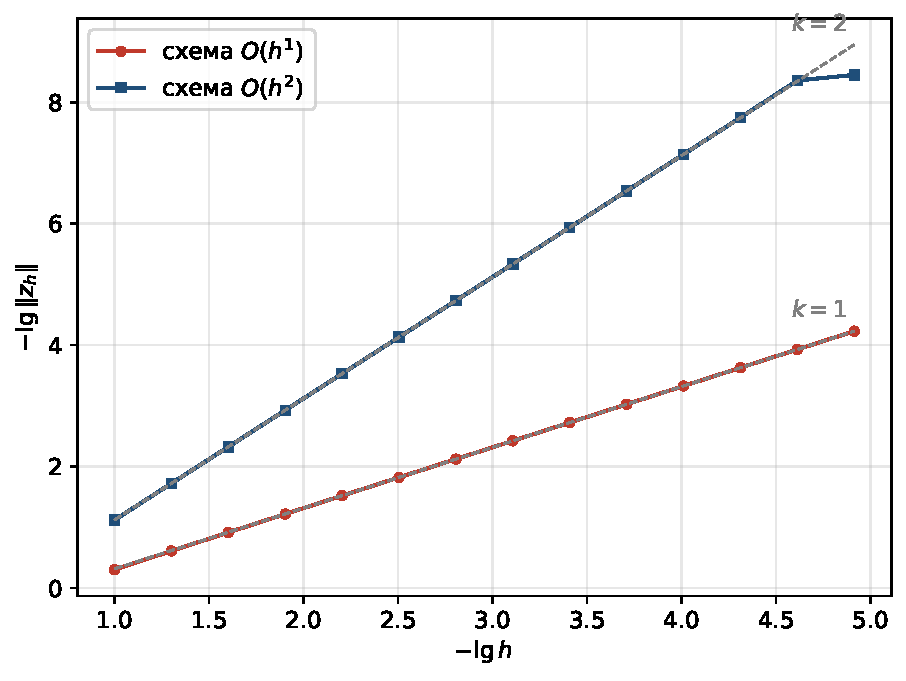
\includegraphics[width=0.8\textwidth]{figures/convergence.pdf}
\caption{Зависимость $-\lg\norm{z_h}$ от $-\lg h$;
штриховые --- эталонные прямые с наклонами $k=1$ и $k=2$}
\label{fig:conv}
\end{figure}

Из табл.~\ref{tab:conv} видно, во сколько раз дороже первый порядок:
погрешность около $6\cdot10^{-5}$ схема A даёт при $n=163\,840$, а схема
B --- уже при $n=640$.

\subsection{Влияние ошибок округления}
\label{sec:round}

Оценка~\eqref{eq:asympt} учитывает только погрешность аппроксимации. На
практике к ней добавляется погрешность округления, которая при
уменьшении $h$ наоборот растёт. Поэтому у полной погрешности есть
минимум, и дальше измельчать сетку бессмысленно.

Все расчёты продублированы в одинарной точности
(\texttt{float32}, $\varepsilon_M\approx1{,}2\cdot10^{-7}$) и в двойной
(\texttt{float64}, $\varepsilon_M\approx2{,}2\cdot10^{-16}$); результаты
--- в табл.~\ref{tab:round} и на рис.~\ref{fig:round}.

\begin{table}[htbp]
\caption{Погрешность $\norm{z_h}$ в одинарной и двойной точности}
\label{tab:round}
\centering
\begin{tabular}{r c c c c}
\toprule
& \multicolumn{2}{c}{схема A, $O(h)$} & \multicolumn{2}{c}{схема B, $O(h^2)$}\\
\cmidrule(lr){2-3}\cmidrule(lr){4-5}
$n$ & double & single & double & single\\
\midrule
20 & $4.98\cdot10^{-1}$ & $4.98\cdot10^{-1}$ & $7.60\cdot10^{-2}$ & $7.60\cdot10^{-2}$ \\
40 & $2.45\cdot10^{-1}$ & $2.45\cdot10^{-1}$ & $1.89\cdot10^{-2}$ & $1.89\cdot10^{-2}$ \\
80 & $1.21\cdot10^{-1}$ & $1.21\cdot10^{-1}$ & $4.73\cdot10^{-3}$ & $4.72\cdot10^{-3}$ \\
160 & $6.05\cdot10^{-2}$ & $6.05\cdot10^{-2}$ & $1.18\cdot10^{-3}$ & $1.18\cdot10^{-3}$ \\
320 & $3.02\cdot10^{-2}$ & $3.02\cdot10^{-2}$ & $2.95\cdot10^{-4}$ & $2.92\cdot10^{-4}$ \\
640 & $1.51\cdot10^{-2}$ & $1.50\cdot10^{-2}$ & $7.38\cdot10^{-5}$ & $1.07\cdot10^{-4}$ \\
1280 & $7.53\cdot10^{-3}$ & $7.93\cdot10^{-3}$ & $1.85\cdot10^{-5}$ & $4.76\cdot10^{-4}$ \\
2560 & $3.77\cdot10^{-3}$ & $6.47\cdot10^{-3}$ & $4.61\cdot10^{-6}$ & $2.82\cdot10^{-3}$ \\
5120 & $1.88\cdot10^{-3}$ & $1.79\cdot10^{-2}$ & $1.15\cdot10^{-6}$ & $1.69\cdot10^{-2}$ \\
10240 & $9.41\cdot10^{-4}$ & $4.58\cdot10^{-1}$ & $2.88\cdot10^{-7}$ & $4.57\cdot10^{-1}$ \\
20480 & $4.71\cdot10^{-4}$ & $8.38\cdot10^{1}$ & $7.21\cdot10^{-8}$ & $8.38\cdot10^{1}$ \\
40960 & $2.35\cdot10^{-4}$ & $8.56\cdot10^{1}$ & $1.79\cdot10^{-8}$ & $8.56\cdot10^{1}$ \\
81920 & $1.18\cdot10^{-4}$ & $8.73\cdot10^{1}$ & $4.38\cdot10^{-9}$ & $8.73\cdot10^{1}$ \\
163840 & $5.88\cdot10^{-5}$ & $8.38\cdot10^{1}$ & $3.54\cdot10^{-9}$ & $8.38\cdot10^{1}$ \\
\bottomrule
\end{tabular}
\end{table}

\begin{figure}[htbp]
\centering
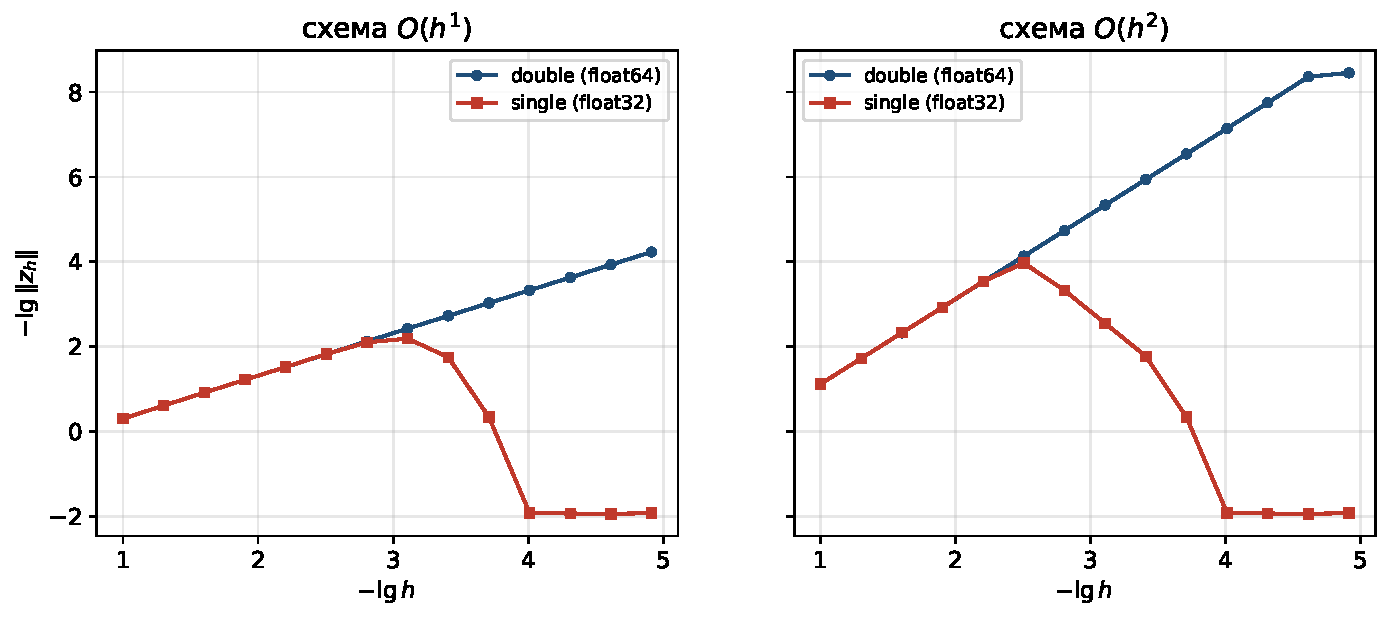
\includegraphics[width=\textwidth]{figures/roundoff.pdf}
\caption{Погрешность в одинарной и двойной точности:
слева схема $O(h)$, справа схема $O(h^2)$}
\label{fig:round}
\end{figure}

В одинарной точности эффект хорошо виден (табл.~\ref{tab:minerr}): для
схемы B минимум погрешности достигается уже при $n=640$, для схемы A ---
при $n=2560$ (у неё собственная погрешность больше и дольше остаётся
главной). При дальнейшем измельчении сетки погрешность растёт, а начиная
примерно с $n=10\,000$ решение разрушается полностью: главный
диагональный элемент $2/h^2+q_i$ при таких $h$ в одинарной точности
округляется до $2/h^2$, слагаемое $q_i$ просто теряется.

В двойной точности при тех же $n$ эффект только начинает проявляться:
в последней строке табл.~\ref{tab:conv} эмпирический порядок схемы B
падает с $2{,}00$ до $0{,}31$.

\begin{table}[htbp]
\caption{Минимальная достижимая погрешность и соответствующее число
разбиений}
\label{tab:minerr}
\centering
\begin{tabular}{c c c c c}
\toprule
& \multicolumn{2}{c}{single (float32)} & \multicolumn{2}{c}{double (float64)}\\
\cmidrule(lr){2-3}\cmidrule(lr){4-5}
схема & $n_{\text{опт}}$ & $\min\norm{z_h}$ & $n_{\text{опт}}$ & $\min\norm{z_h}$\\
\midrule
$O(h)$ & 2560 & $6.47\cdot10^{-3}$ & $\ge 163840$ & $5.88\cdot10^{-5}$ \\
$O(h^2)$ & 640 & $1.07\cdot10^{-4}$ & $\ge 163840$ & $3.54\cdot10^{-9}$ \\
\bottomrule
\end{tabular}
\end{table}

\subsection{Число разбиений для заданной точности}

Здесь ограничиваться сетками из последовательности удвоений уже не
нужно: погрешность монотонно убывает с ростом $n$, поэтому наименьшее
подходящее $n$ находится двоичным поиском по отрезку $2\le n\le 200\,000$
(около 18 решений задачи на каждое значение $\varepsilon$). Результаты ---
в табл.~\ref{tab:eps}, расчёт в двойной точности.

\begin{table}[htbp]
\caption{Число разбиений $n$, необходимое для достижения точности
$\varepsilon$}
\label{tab:eps}
\centering
\begin{tabular}{c c c c c}
\toprule
& \multicolumn{2}{c}{схема A, $O(h)$} & \multicolumn{2}{c}{схема B, $O(h^2)$}\\
\cmidrule(lr){2-3}\cmidrule(lr){4-5}
$\varepsilon$ & $n$ & $\norm{z_h}$ & $n$ & $\norm{z_h}$\\
\midrule
$10^{-2}$ & 965 & $9.99\cdot10^{-3}$ & 56 & $9.65\cdot10^{-3}$ \\
$10^{-3}$ & 9638 & $1.00\cdot10^{-3}$ & 174 & $9.99\cdot10^{-4}$ \\
$10^{-4}$ & 96371 & $1.00\cdot10^{-4}$ & 550 & $9.99\cdot10^{-5}$ \\
$10^{-5}$ & --- & --- & 1739 & $1.00\cdot10^{-5}$ \\
$10^{-6}$ & --- & --- & 5499 & $1.00\cdot10^{-6}$ \\
\bottomrule
\end{tabular}
\end{table}

Числа хорошо согласуются с теорией. Для схемы A из $\norm{z_h}\approx Ch$
следует $n\sim\varepsilon^{-1}$: переход к следующей строке таблицы
увеличивает $n$ ровно в 10 раз ($965\to9638\to96\,371$). Для схемы B из
$\norm{z_h}\approx Ch^2$ следует $n\sim\varepsilon^{-1/2}$, то есть рост
в $\sqrt{10}\approx3{,}16$ раза ($56\to174\to550\to1739\to5499$).

Поэтому отношение затрат растёт как $\varepsilon^{-1/2}$: при
$\varepsilon=10^{-2}$ схеме A нужно в 17 раз больше узлов, при
$\varepsilon=10^{-3}$ --- в 55 раз, при $\varepsilon=10^{-4}$ --- в 175
раз. Точность $10^{-5}$ потребовала бы от схемы A порядка $10^{6}$ узлов
(это за пределами взятого ограничения $n\le200\,000$), тогда как схеме B
хватает 1739.

\subsection{Оценка погрешности по методу Рунге}
\label{sec:runge}

Пусть схема имеет порядок $k$, а $v_h$ и $v_{h/2}$ --- решения на сетках
с шагами $h$ и $h/2$. В общих узлах
\[
u-v_h = C h^k+O(h^{k+1}),\qquad
u-v_{h/2} = C\Bigl(\frac h2\Bigr)^{k}+O(h^{k+1}).
\]
Константа $C$ неизвестна, но её можно исключить. Вычтем второе равенство
из первого; точное решение $u$ при этом сокращается, и остаются только
величины, которые мы умеем считать:
\[
v_{h/2}-v_h=(u-v_h)-(u-v_{h/2})
 =Ch^k\Bigl(1-\frac1{2^k}\Bigr)+O(h^{k+1})
 =\frac{Ch^k}{2^k}\,(2^k-1)+O(h^{k+1}).
\]
Но $\dfrac{Ch^k}{2^k}=C\Bigl(\dfrac h2\Bigr)^{k}$ --- это как раз главный
член погрешности на мелкой сетке. Значит
\[
u-v_{h/2}=\frac{Ch^k}{2^k}+O(h^{k+1})
         =\frac{v_{h/2}-v_h}{2^k-1}+O(h^{k+1}),
\]
и мы получаем оценку Рунге погрешности решения на мелкой сетке
\begin{equation}\label{eq:runge}
R:=\frac{v_{h/2}-v_h}{2^k-1}\;\approx\; u-v_{h/2},
\end{equation}
а вместе с ней и уточнённое решение
\begin{equation}\label{eq:rich}
\tilde v = v_{h/2}+\frac{v_{h/2}-v_h}{2^k-1}.
\end{equation}
Оценка~\eqref{eq:runge} не использует точного решения, поэтому годится и
для реальных задач.

Результаты --- в табл.~\ref{tab:runge1} и~\ref{tab:runge2} и на
рис.~\ref{fig:runge}. Отношение $\norm{R}/\norm{z_{h/2}}$ показывает,
насколько хороша оценка: с измельчением сетки оно стремится к единице
($1{,}034\to1{,}000$ для схемы A и $1{,}006\to1{,}000$ для схемы B).

\begin{table}[htbp]
\caption{Метод Рунге для схемы A ($k=1$)}
\label{tab:runge1}
\centering
\begin{tabular}{r c c c c c}
\toprule
$n$ & $\norm{R}$ & $\norm{z_{h/2}}$ &
$\dfrac{\norm{R}}{\norm{z_{h/2}}}$ & $\norm{u-\tilde v}$ &
порядок\\
\midrule
20 & $2.53\cdot10^{-1}$ & $2.45\cdot10^{-1}$ & 1.034 & $4.49\cdot10^{-2}$ & --- \\
40 & $1.23\cdot10^{-1}$ & $1.21\cdot10^{-1}$ & 1.017 & $1.12\cdot10^{-2}$ & 2.00 \\
80 & $6.10\cdot10^{-2}$ & $6.05\cdot10^{-2}$ & 1.008 & $2.81\cdot10^{-3}$ & 2.00 \\
160 & $3.03\cdot10^{-2}$ & $3.02\cdot10^{-2}$ & 1.004 & $7.03\cdot10^{-4}$ & 2.00 \\
320 & $1.51\cdot10^{-2}$ & $1.51\cdot10^{-2}$ & 1.002 & $1.76\cdot10^{-4}$ & 2.00 \\
640 & $7.54\cdot10^{-3}$ & $7.53\cdot10^{-3}$ & 1.001 & $4.40\cdot10^{-5}$ & 2.00 \\
1280 & $3.77\cdot10^{-3}$ & $3.77\cdot10^{-3}$ & 1.000 & $1.10\cdot10^{-5}$ & 2.00 \\
2560 & $1.88\cdot10^{-3}$ & $1.88\cdot10^{-3}$ & 1.000 & $2.75\cdot10^{-6}$ & 2.00 \\
5120 & $9.41\cdot10^{-4}$ & $9.41\cdot10^{-4}$ & 1.000 & $6.87\cdot10^{-7}$ & 2.00 \\
\bottomrule
\end{tabular}
\end{table}

\begin{table}[htbp]
\caption{Метод Рунге для схемы B ($k=2$)}
\label{tab:runge2}
\centering
\begin{tabular}{r c c c c c}
\toprule
$n$ & $\norm{R}$ & $\norm{z_{h/2}}$ &
$\dfrac{\norm{R}}{\norm{z_{h/2}}}$ & $\norm{u-\tilde v}$ &
порядок\\
\midrule
20 & $1.90\cdot10^{-2}$ & $1.89\cdot10^{-2}$ & 1.006 & $3.65\cdot10^{-4}$ & --- \\
40 & $4.73\cdot10^{-3}$ & $4.73\cdot10^{-3}$ & 1.002 & $2.23\cdot10^{-5}$ & 4.03 \\
80 & $1.18\cdot10^{-3}$ & $1.18\cdot10^{-3}$ & 1.000 & $1.39\cdot10^{-6}$ & 4.01 \\
160 & $2.95\cdot10^{-4}$ & $2.95\cdot10^{-4}$ & 1.000 & $8.69\cdot10^{-8}$ & 4.00 \\
320 & $7.38\cdot10^{-5}$ & $7.38\cdot10^{-5}$ & 1.000 & $5.43\cdot10^{-9}$ & 4.00 \\
640 & $1.85\cdot10^{-5}$ & $1.85\cdot10^{-5}$ & 1.000 & $3.39\cdot10^{-10}$ & 4.00 \\
1280 & $4.61\cdot10^{-6}$ & $4.61\cdot10^{-6}$ & 1.000 & $2.09\cdot10^{-11}$ & 4.02 \\
\bottomrule
\end{tabular}
\end{table}

\begin{figure}[htbp]
\centering
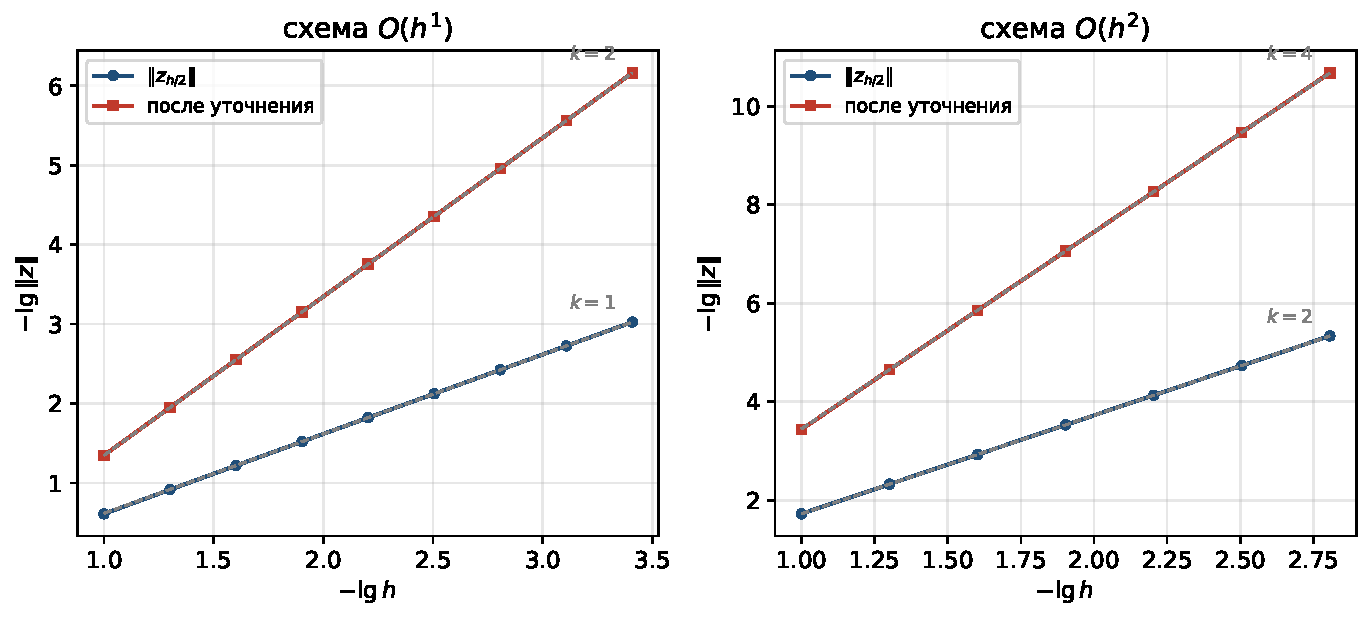
\includegraphics[width=\textwidth]{figures/runge.pdf}
\caption{Погрешность решения на мелкой сетке и после уточнения;
штриховые --- эталонные прямые}
\label{fig:runge}
\end{figure}

Уточнение~\eqref{eq:rich} заметно повышает точность. Формула~\eqref{eq:rich}
убирает главный член $Ch^k$, поэтому порядок уточнённого решения
определяется тем, какой член в разложении погрешности идёт следующим.

Для схемы A следующий член --- $h^2$, и уточнённое решение имеет второй
порядок; это и получено в табл.~\ref{tab:runge1}. Для схемы B измеренный
порядок равен 4 (табл.~\ref{tab:runge2}), то есть члена $h^3$ в
разложении нет.

Для внутренних узлов это прямо следует из~\eqref{eq:psi}: невязка
содержит только чётные степени $h$, потому что в центральных
разностях~\eqref{eq:d2} и~\eqref{eq:d1} нечётные члены сокращаются.
С краевыми уравнениями схемы B всё не так очевидно. Если подставить в
левое краевое уравнение~\eqref{eq:bc2a} точное решение и разложить $u_1$
по формуле~\eqref{eq:taylor_inner}, то члены порядка $1$ и $h$
сокращаются (именно так уравнение и строилось), а дальше остаётся
\begin{equation}\label{eq:bc_resid}
\tau_a=-\alpha_a\Bigl(\frac{h^2}{6}\,u'''(a)+\frac{h^3}{24}\,u^{(4)}(a)\Bigr)
       +O(h^4),
\end{equation}
и точно так же на правом конце. Нечётная степень $h^3$ здесь
присутствует, так что заранее рассчитывать на четвёртый порядок нельзя:
из~\eqref{eq:bc_resid} гарантируется только третий.

Тем не менее в глобальной погрешности член $h^3$ не появляется. Причина в
том, что коэффициенты самих краевых уравнений тоже зависят от $h$
(множители $D_a$, $D_b$ и слагаемые вида $\alpha h q/2$), и поправка от
них гасит вклад $h^3$-части невязки. Аккуратно выписывать это
громоздко, поэтому проверим численно. Если
$z(h)=c_kh^k+c_{k+1}h^{k+1}+\dots$, то комбинация
\begin{equation}\label{eq:evencheck}
d(h):=z(h)-2^{k}z(h/2)
\end{equation}
убирает главный член, и отношение $d(h)/d(h/2)$ равно $2^{k+1}$, если
следующий член нечётный, и $2^{k+2}$, если нечётного члена нет.
Погрешность бралась в одном узле $x=a$ (на границе, где и стоит вопрос),
чтобы не переключаться между разными точками максимума. Результат --- в
табл.~\ref{tab:even}: для схемы A отношение равно 4, то есть
$k=1$ и следующий член $h^2$; для схемы B --- 16, то есть $k=2$ и
следующий член сразу $h^4$. Тот же порядок 4 получается и для другого
точного решения ($u^*=e^{x}\cos x$), так что дело не в удачном выборе
$u^*$.

\begin{table}[htbp]
\caption{Проверка~\eqref{eq:evencheck}: какие степени $h$ входят в
разложение погрешности (узел $x=a$)}
\label{tab:even}
\centering
\begin{tabular}{r c c c c}
\toprule
& \multicolumn{2}{c}{схема A, $k=1$} & \multicolumn{2}{c}{схема B, $k=2$}\\
\cmidrule(lr){2-3}\cmidrule(lr){4-5}
$n$ & $d(h)$ & $d(h)/d(h/2)$ & $d(h)$ & $d(h)/d(h/2)$\\
\midrule
40 & $-2.04\cdot10^{-3}$ & 4.14 & $4.26\cdot10^{-5}$ & 16.17 \\
80 & $-4.92\cdot10^{-4}$ & 4.10 & $2.64\cdot10^{-6}$ & 16.04 \\
160 & $-1.20\cdot10^{-4}$ & 4.05 & $1.64\cdot10^{-7}$ & 16.01 \\
320 & $-2.96\cdot10^{-5}$ & 4.03 & $1.03\cdot10^{-8}$ & 16.06 \\
\midrule
\multicolumn{1}{r}{ожидается} & \multicolumn{2}{c}{$2^{k+1}=4$}
 & \multicolumn{2}{c}{$2^{k+2}=16$}\\
\bottomrule
\end{tabular}
\end{table}

Таблица~\ref{tab:runge2} обрывается на $n=1280$: при больших $n$
погрешность уточнённого решения ($\sim10^{-12}$) сравнивается с
погрешностью округления и измеренный порядок теряет смысл.

\section{Выводы}

\begin{enumerate}
\item Для краевой задачи третьего рода построены и реализованы две
разностные схемы, отличающиеся только аппроксимацией краевых условий.
Обе дают систему линейных алгебраических уравнений (СЛАУ) с
трёхдиагональной матрицей, которая решается методом прогонки.

\item Теоретические порядки точности подтвердились: эмпирический
порядок~\eqref{eq:order} равен $1{,}00$ для схемы A и $2{,}00$ для схемы
B, графики $-\lg\norm{z_h}$ от $-\lg h$ параллельны эталонным прямым с
наклонами $k=1$ и $k=2$.

\item Аппроксимация краевых условий определяет порядок всей схемы:
односторонняя разность на границе понижает его до первого, хотя внутри
области схема второго порядка. Переход к схеме B не усложняет структуру
матрицы, но сокращает нужное для достижения требуемой точности число
узлов в десятки и сотни раз (табл.~\ref{tab:eps}).

\item Обнаружен эффект насыщения погрешности. В одинарной точности
минимум достигается при $n=640$ (схема B) и $n=2560$ (схема A), дальше
измельчение сетки только вредит, а при $n\gtrsim 10\,000$ решение
разрушается. В двойной точности при тех же сетках это видно только по
падению эмпирического порядка схемы B на последнем шаге.

\item Оценка погрешности по методу Рунге оказалась точной: её отношение
к истинной погрешности стремится к единице. Уточнение по
формуле~\eqref{eq:rich} повышает порядок с 1 до 2 для схемы A и с 2 до 4
для схемы B; при $n=1280$ уточнённое решение даёт погрешность
$2{,}1\cdot10^{-11}$ против $4{,}6\cdot10^{-6}$ у самой схемы B.
\end{enumerate}

\end{document}
